\documentclass[10pt,a4paper]{article}
\usepackage[margin=23mm,top=20mm,bottom=20mm]{geometry}
\usepackage[T1]{fontenc}
\usepackage{amsmath,amssymb,booktabs,xcolor,graphicx,hyperref}
\graphicspath{{../figures/}}
\hypersetup{colorlinks=true,linkcolor=blue!45!black,urlcolor=blue!45!black,pdftitle={Double Descent in Linear Models},pdfauthor={Stela Mile}}
\definecolor{bluecurve}{RGB}{30,105,165}
\definecolor{orangecurve}{RGB}{224,110,25}
\definecolor{greencurve}{RGB}{28,128,82}
\definecolor{blueband}{RGB}{205,225,240}
\definecolor{orangeband}{RGB}{251,226,204}
\definecolor{grid}{RGB}{220,224,228}
\setlength{\parindent}{0pt}
\setlength{\parskip}{6pt}
\setlength{\tabcolsep}{6pt}
\renewcommand{\arraystretch}{1.2}
\newcommand{\pageheading}[1]{\section*{#1}}
\begin{document}
{\Large\bfseries Double Descent in Linear Models}\par
{\large Minimum-norm least squares and ridge regression}\par
\textbf{Stela Mile}\quad |\quad Statistical Methods for Machine Learning\par
Assignment 4\quad |\quad A.Y. 2025/26\quad |\quad 29 October 2026

\pageheading{1. Research question and main findings}
Classical accounts of generalization emphasize a trade-off: increasing model complexity can reduce approximation error while increasing estimation error. Beyond the capacity needed to fit the training set exactly, test error can decline again. This is the double-descent phenomenon discussed by Belkin et al.\ [1]. This project investigates that behavior in linear regression by holding the number of training observations fixed and varying the number of available features.

\textbf{Abstract.} Minimum-norm least squares and ridge regression are implemented with explicit NumPy linear algebra and evaluated on noisy synthetic linear data and a real-world BlogFeedback regression task. The synthetic experiment exhibits a pronounced interpolation spike followed by a second descent. Ridge substantially suppresses that spike. The real-world experiment reaches numerical interpolation, but its predictive performance is unstable. Across repeated subsets, a median peak and decline coexist with weak performance against a constant baseline. These findings support a distinction between identifying interpolation, observing a second descent, and achieving useful prediction.

\begin{center}
\begin{tabular}{p{0.23\linewidth}p{0.32\linewidth}p{0.32\linewidth}}
\toprule
 & Synthetic data & BlogFeedback \\
\midrule
Fixed training size & 150 & 80 \\
Test observations & 1,000 per run & 214, fixed later date \\
Repeated seeds & 0--29 & 0--19 \\
Observed interpolation & At $d=150$ & $d=80$--$93$ in repetitions \\
Main pattern & Clear double descent & Mixed evidence; high instability \\
Regularization & Suppresses the spike & Improves on unstable least squares \\
Practical caveat & Largest model is not best & Final ridge models lose to baseline \\
\bottomrule
\end{tabular}
\end{center}

\textbf{Scope.} The experiments are diagnostic sweeps, not a model-selection exercise. The test curves are used to study behavior, not to choose the dimension or regularization strength for deployment. No claim is made that these linear experiments reproduce the models or full empirical scope of the reference paper.

\textbf{Evidence.} Every numerical statement below is derived from the executed notebooks and accompanying JSON results. Linear and logarithmic views are retained in the repository; the report uses logarithmic error plots where large spikes would otherwise obscure the ridge and baseline curves.

\newpage
\pageheading{2. Models, loss, and numerical interpolation}
For a design matrix $X\in\mathbb{R}^{n\times d}$ and labels $y\in\mathbb{R}^n$, least squares minimizes the unnormalized sum of squared errors:
\[
\widehat w\in\arg\min_w\|Xw-y\|_2^2.
\]
When the minimizer is not unique, the implementation chooses the solution with smallest Euclidean norm. Given a reduced singular value decomposition $X=U\Sigma V^\top$, it computes
\[
\widehat w=V_K\Sigma_K^{-1}U_K^\top y,
\qquad K=\{j:s_j>10^{-10}s_1\}.
\]
The cutoff prevents division by numerically negligible singular values. This is a truncated numerical pseudoinverse; the numerical rank, and hence the fitted solution, depends on the stated tolerance. The real-world diagnostic table uses the same retained singular values as the solver, rather than a separate default rank threshold.

Ridge regression minimizes
\[
\|Xw-y\|_2^2+\alpha\|w\|_2^2,\qquad\alpha>0,
\]
and solves the linear system
\[
(X^\top X+\alpha I)\widehat w_\alpha=X^\top y.
\]
The code uses \texttt{numpy.linalg.solve}, not an explicit matrix inverse. The objective uses the sum of errors, so $\alpha$ is not the penalty coefficient of an objective normalized by $1/n$. Its spectral action replaces the factor $1/s_j$ by $s_j/(s_j^2+\alpha)$, limiting the amplification associated with small singular values. The implementation and normalization match the ridge formulation in the supplied course notes [3].

\textbf{Error metric.} Both train and test errors are means:
\[
\operatorname{MSE}(y,\widehat y)=\frac{1}{m}\sum_{i=1}^m(y_i-\widehat y_i)^2.
\]
Synthetic MSE is on the original label scale. BlogFeedback MSE is on $\log(1+y)$; centering does not change the error when the training mean is restored to predictions.

\textbf{Interpolation diagnostic.} The real-world implementation evaluates
\[
\rho_d=\frac{\|y-X_d\widehat w_d\|_2}
{\max(\|y\|_2,\epsilon_{\rm machine})}
\]
and records the first dimension with $\rho_d<10^{-8}$. Interpolation is therefore observed from the training residual, not inferred from a large parameter count or a test-error spike. Centering the real-world columns restricts their rank to at most $n-1$; a centered target can still be interpolated if it lies in their column space. Neither $d=n$ nor rank alone is a sufficient diagnostic in rank-deficient data.

\newpage
\pageheading{3. Datasets and evaluation protocol}
\textbf{Synthetic regression.} Each run draws independent standard Gaussian feature matrices with 150 training rows, 1,000 test rows, and 400 columns. Labels are generated once from all 400 features:
\[
y=X\beta+\varepsilon,\quad\varepsilon\sim\mathcal N(0,\sigma^2I),
\qquad \beta_j\propto s_j e^{-0.02j},\ j=0,\ldots,399,
\]
where $s_j\in\{-1,1\}$ are random signs and $\|\beta\|_2=1$. Thus the population signal variance is one. The main experiment uses $\sigma=0.5$, corresponding to noise variance 0.25.

The models take prefixes of the same matrices. Labels, noise, and coefficient vector do not change as $d$ varies within a run. Early features deliberately carry more signal, so adding features initially reduces omitted-variable error. Thirty seeds generate independent problems. Least squares and all four ridge strengths, $\alpha\in\{0.01,0.1,1,10\}$, use identical data within each seed. A dense set of dimensions near 150 resolves the interpolation spike; the sweep continues to 400.

\textbf{Real-world regression.} BlogFeedback [2] provides a training file with 52,397 observations and 280 predictors. The target is a future comment count. The experiment uses the final provided test file, dated 31 March 2012, containing 214 observations. This preserves the official separation of training and test files, while limiting the evaluation to one test date. The other 59 test files are not pooled.

For each run, 80 observations are sampled without replacement from the official training file. The target is transformed with $\log(1+y)$ because of its skew. Predictors are randomly ordered, standardized using only the selected training rows, and columns with zero training variance are removed. Targets are centered with the training mean; this is equivalent to fitting an unpenalized intercept. All preprocessing is applied unchanged to the held-out file.

\textbf{Why a small fixed sample?} The aim is to cross interpolation within the available feature set, rather than to train the most accurate predictor. An earlier $n=150$ setup remained rank deficient and did not interpolate. Reducing the fixed size to 80 made interpolation accessible. This was an exploratory design revision, not an independent confirmatory experiment. Seed 42 is retained for illustration; seeds 0--19 provide repeated diagnostics without replacing unfavorable runs.

Every usable dimension is evaluated in each real-world run. Unsupported dimensions are stored as missing values, not silently truncated. Aggregate plots use only dimensions available in all 20 runs, namely 1--149 in the verified execution. Ridge uses $\alpha=1$. The baseline predicts the mean of that run's training log-targets and never uses the test mean.

\newpage
\pageheading{4. Synthetic results: a clear interpolation spike}
\begin{center}
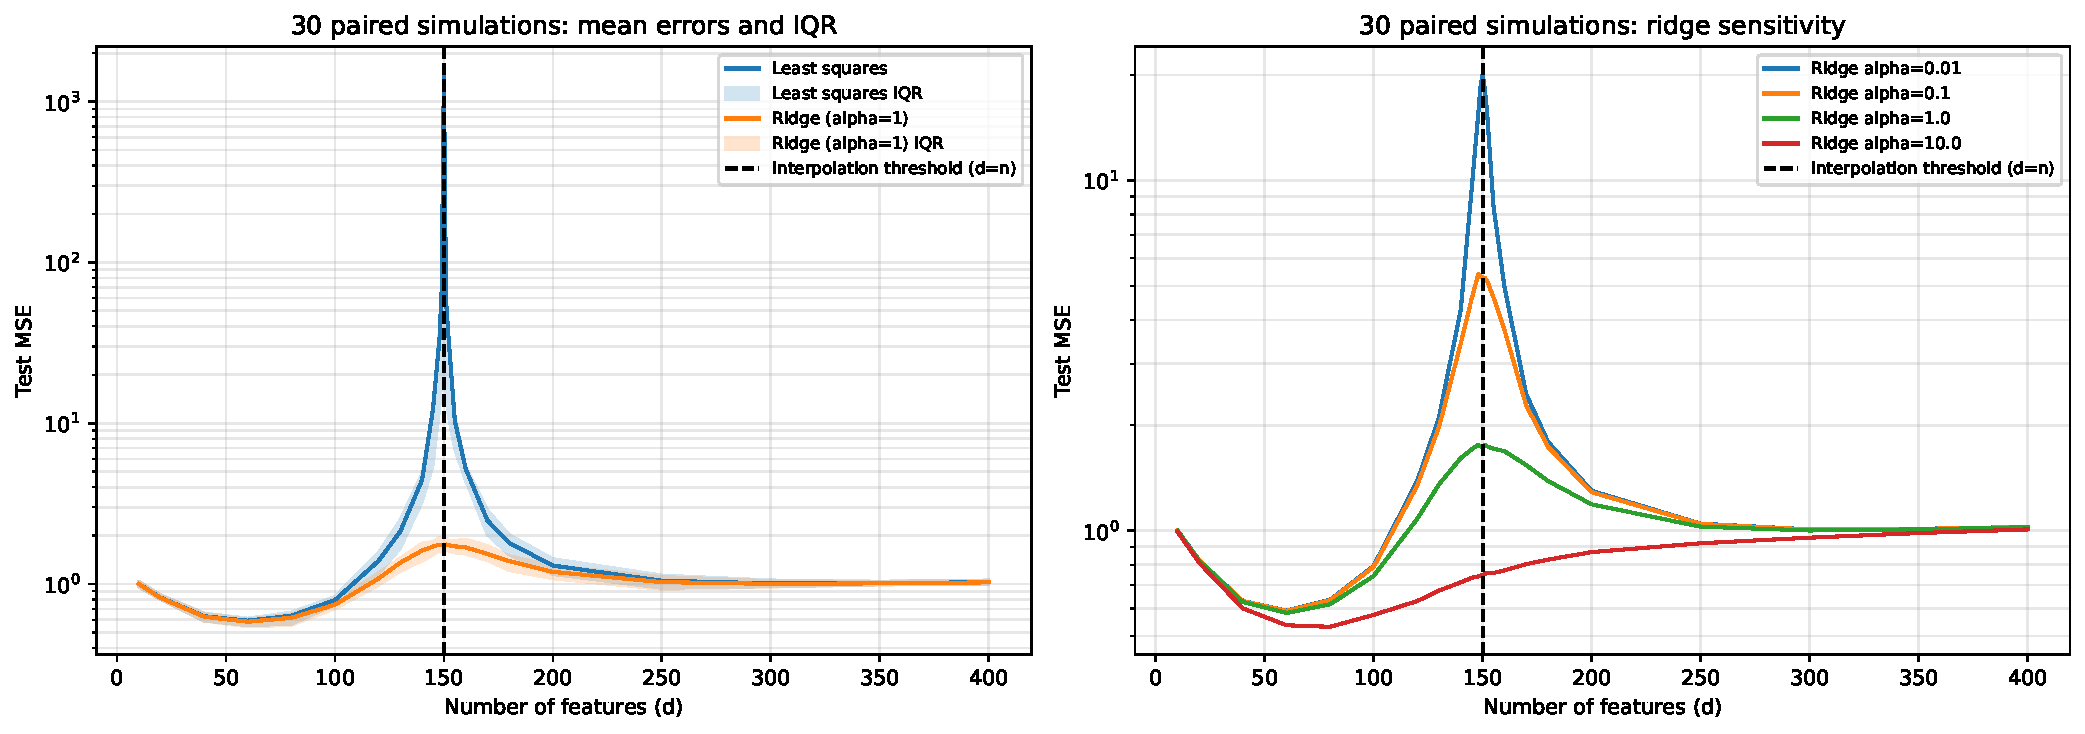
\includegraphics[width=\linewidth,height=0.23\textheight,keepaspectratio]{synthetic_06.pdf}
\end{center}
{\small\textit{Figure 1.} Paired mean errors and IQRs (left), and ridge sensitivity (right), across the same 30 synthetic problems. The dashed line marks $d=n=150$.}


The least-squares curve initially falls, rises toward interpolation, and declines again as additional features are introduced. The mean test error at $d=150$ is about 1,477.95, compared with about 1.026 at $d=400$. Training error reaches numerical zero in the interpolating regime. This is a clear empirical instance of double descent under the specified data-generating process.

However, the best observed pre-interpolation mean is about 0.591 at $d=60$, below the final error. A second descent does not imply that the largest model is the best model. Once the informative early features have been included, adding further coordinates also changes the bias of the minimum-norm solution.

Ridge with $\alpha=1$ lowers mean error at $d=150$ to about 1.725. At $d=400$, ridge and least squares are nearly identical, about 1.024 and 1.026. Its largest benefit here is near the ill-conditioned interpolation transition. The four-strength sensitivity plot in the notebook shows that stronger regularization suppresses the spike more aggressively; those test curves are descriptive, not a tuning procedure.

Means near the interpolation threshold can be sensitive to extreme realizations. The notebook therefore also displays interquartile ranges. An empirical mean need not lie inside the middle-50\% band; the band is not a confidence interval for that mean.

\subsection*{Gradient descent and early stopping}
Zero-initialized gradient descent uses the same seed-42 data and dimension sweep, optimizing half the sum-of-squares objective with $\eta=0.9/(s_{\max}^2+\alpha)$. Fixed 20, 200 and 2,000-step runs show early stopping. Zero initialization keeps unregularized iterates in the row space, explaining convergence to the minimum-norm fit. Finite iterations damp slowly learned singular directions and provide implicit regularization; they are not identical to ridge.
\begin{center}
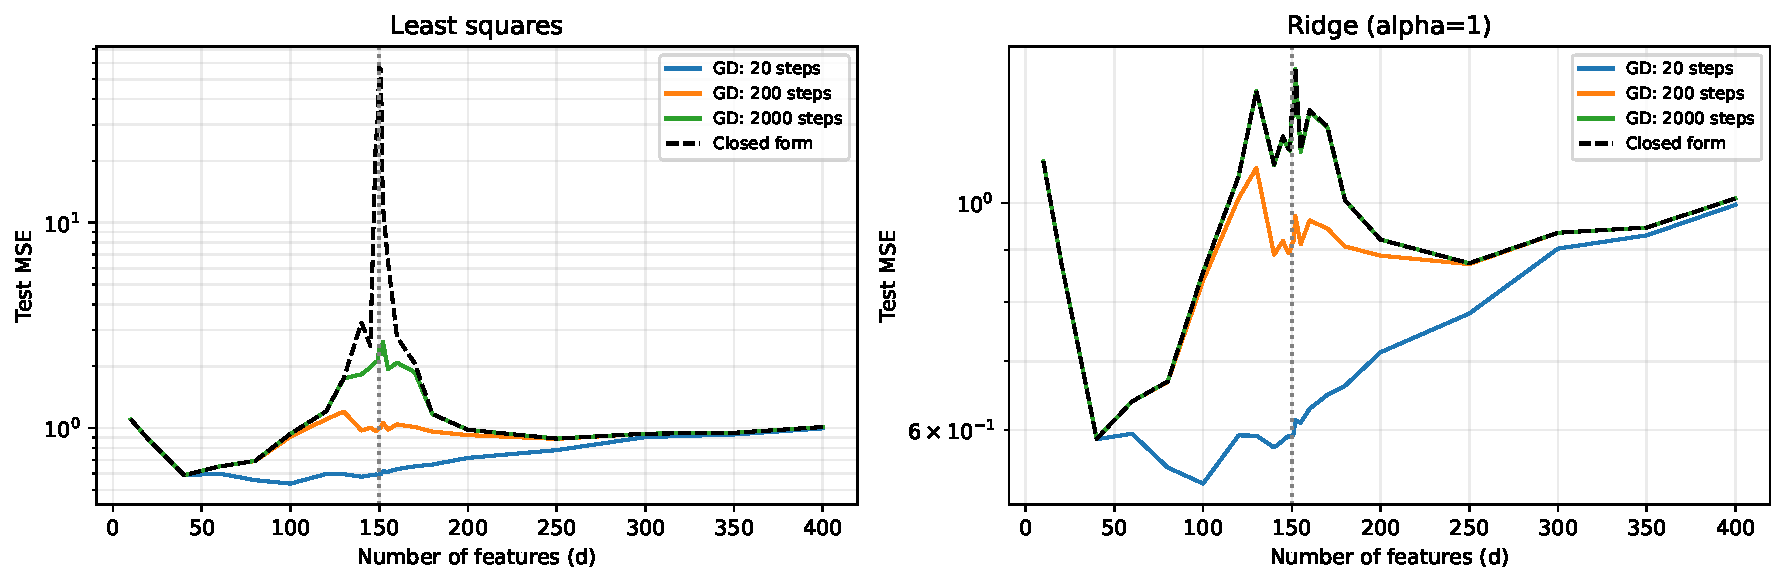
\includegraphics[width=\linewidth,height=.18\textheight,keepaspectratio]{synthetic_gd.pdf}
\end{center}
{\small\textit{Figure 2.} Finite-step GD versus closed form, with and without explicit ridge regularization; all curves use seed 42.}

Separate training-only checks report coefficient differences. At $d=200$, unregularized GD reaches $\|w_{GD}-w_{SVD}\|_2\approx1.02\times10^{-8}$ after 2,400 steps; at $d=400$, the difference is $6.92\times10^{-11}$ after 300 steps. At $d=150$, even 20,000 steps leave a difference of 5.46 (relative difference 0.733), so convergence is not claimed there. Ridge with $\alpha=1$ reaches the $10^{-8}$ relative coefficient tolerance in the checked dimensions, including $d=150$ after 9,600 steps.

\newpage
\pageheading{5. Real-world interpolation and an unstable illustration}
\begin{center}
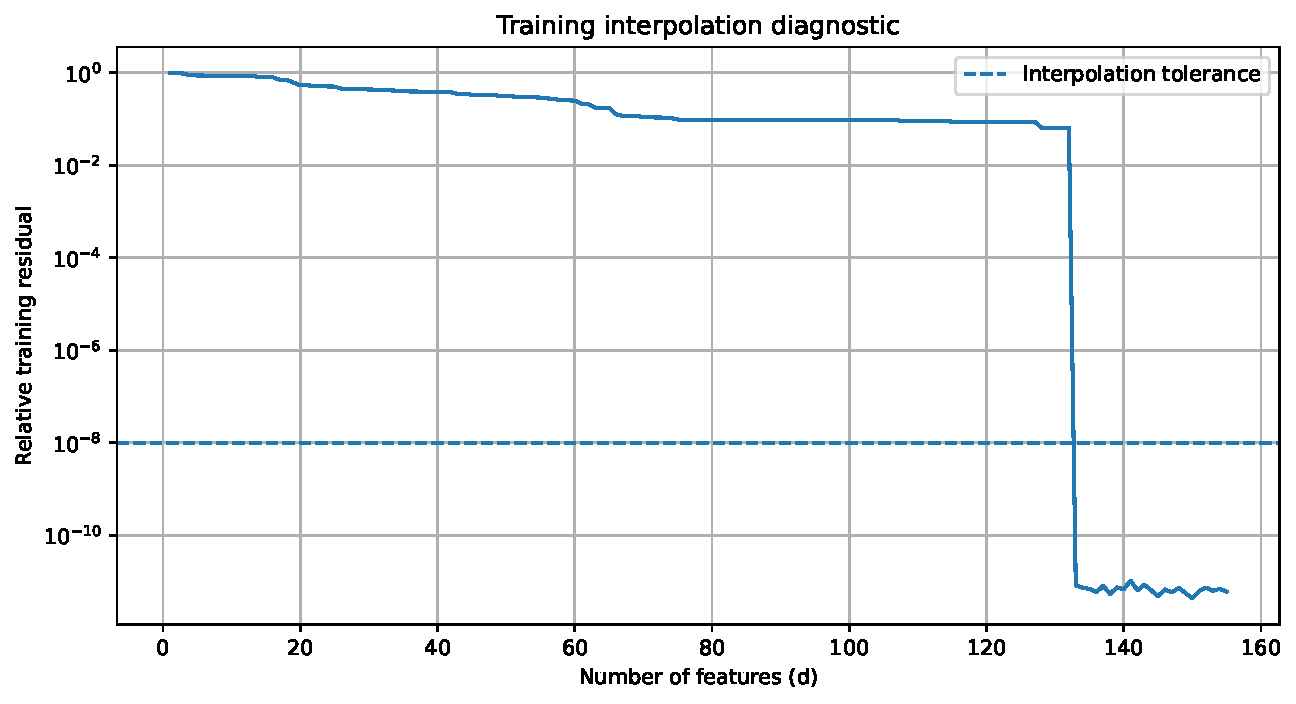
\includegraphics[width=\linewidth,height=0.25\textheight,keepaspectratio]{real_world_01.pdf}
\end{center}
{\small\textit{Figure 3.} The relative training residual falls below $10^{-8}$ at $d=133$ in the seed-42 run. The dashed vertical line marks that observed event.}

The seed-42 test curves are shown with the repeated-run medians in Figure 4.

The seed-42 subset retains 155 nonconstant predictors. Its final training MSE is approximately $4.12\times10^{-23}$, confirming numerical interpolation. Nevertheless, final test MSE is about $4.31\times10^7$ for least squares and 13.37 for ridge, versus 1.14 for the baseline. This run does not demonstrate a convincing second descent. It is retained because replacing it with a favorable seed would conceal important instability. Tiny training residuals alone do not establish good generalization.

\newpage
\pageheading{6. Real-world repetitions and ridge selection}
\begin{center}
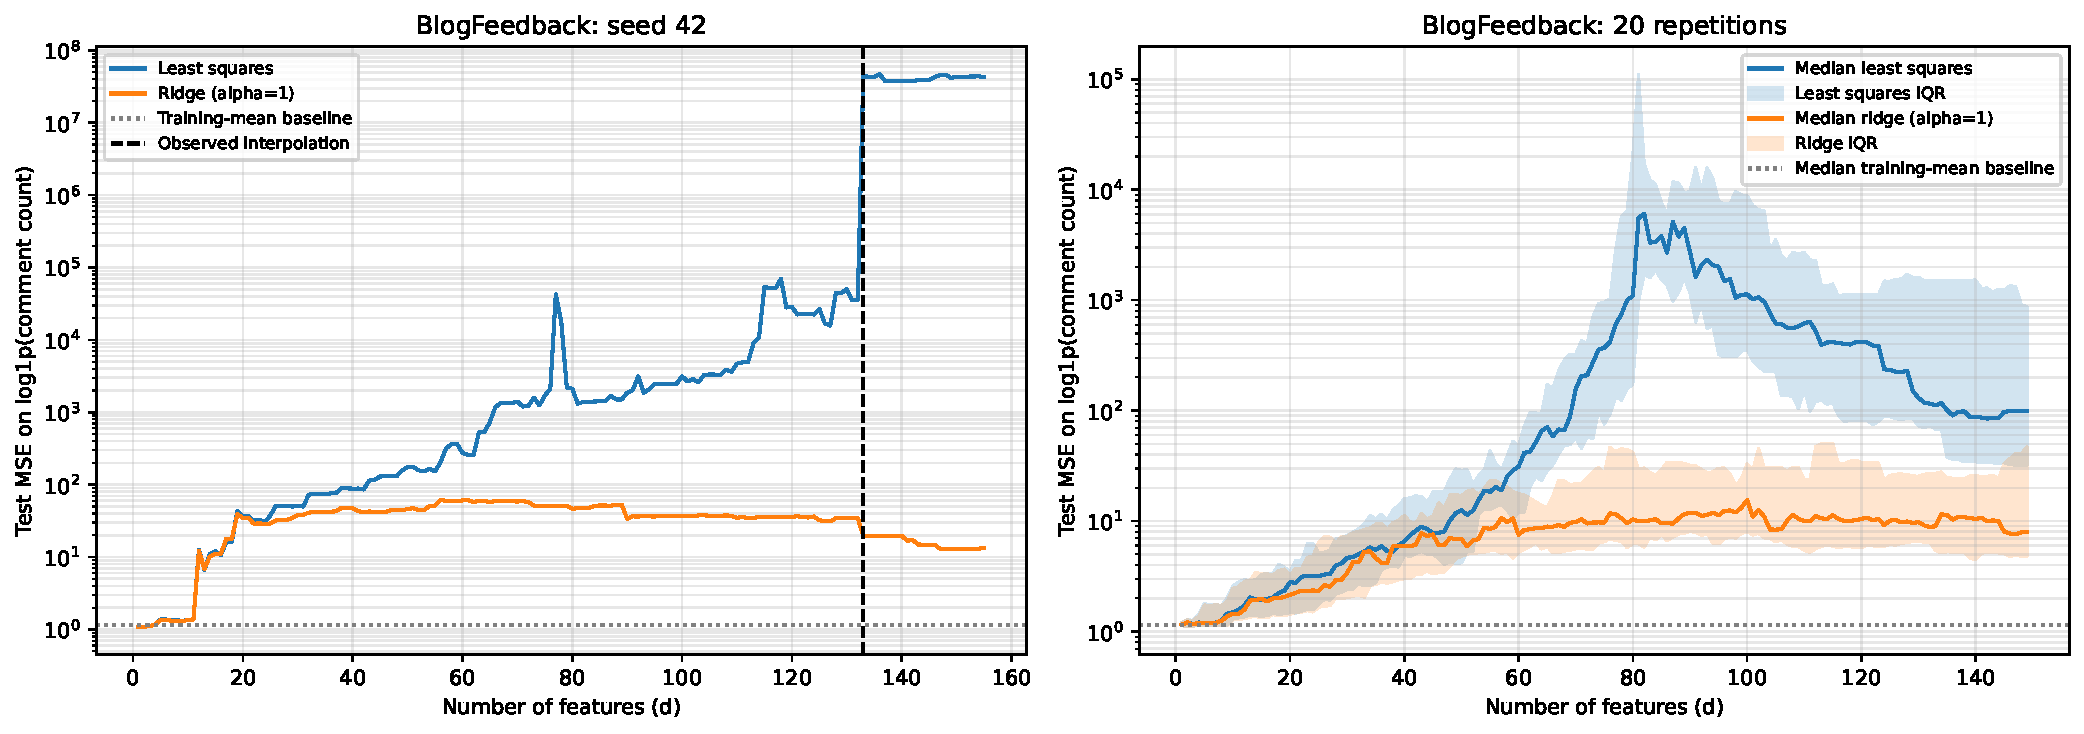
\includegraphics[width=\linewidth,height=.20\textheight,keepaspectratio]{real_world_08.pdf}
\end{center}
{\small\textit{Figure 4.} Seed-42 test errors (left) and repeated-run medians with IQRs (right). These use the original effective-feature axis and fixed $\alpha=1$.}

All 20 original repetitions interpolate at dimensions 80--93. Median least-squares MSE peaks at 6,063.209 at $d=82$ and declines to 99.277 at the final common effective dimension, $d=149$. Ridge's median is 7.903 there, versus 1.147 for the baseline; it wins in 0/20 paired comparisons. The curve lacks a clean initial descent. IQRs describe sensitivity to sampled training rows and ordering, not uncertainty across independent test dates. The seed-42 run remains an unfavorable illustration rather than being replaced.

\subsection*{Five-fold cross-validation inside training data}
A separate extension sweeps $\alpha\in\{0.01,0.1,1,10,100\}$ and selects alpha by five-fold validation within each 80-row training subset, separately at fixed raw prefix lengths 10, 20, 40, 60, 80, 100, 120, 160, 200, 240 and 280. Each fitting fold learns its own constant-column mask, means, scales and target mean. The validation fold is used only for scoring; the official test file is not used for selection. The selected model is refitted on all 80 training rows.
\begin{center}
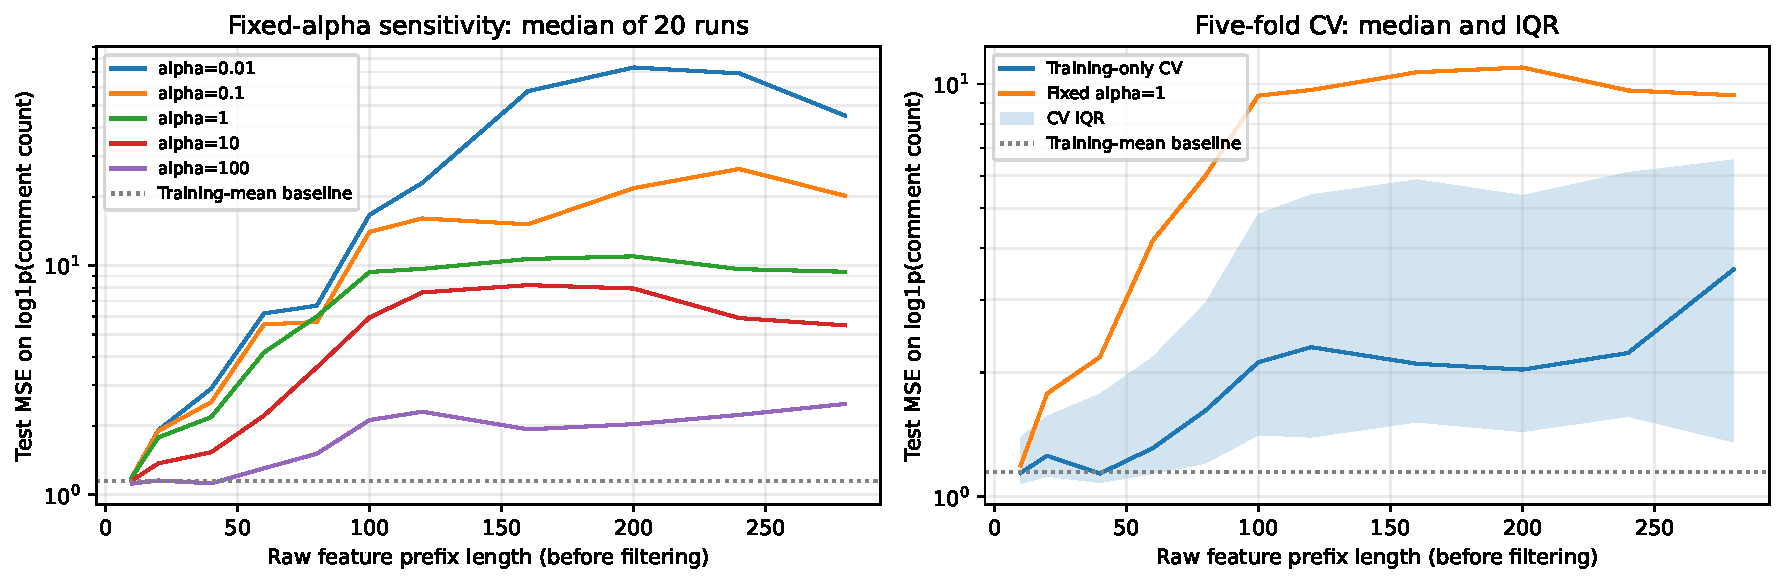
\includegraphics[width=\linewidth,height=.20\textheight,keepaspectratio]{real_ridge_cv.pdf}
\end{center}
{\small\textit{Figure 5.} Fixed-alpha sensitivity and training-only CV across 20 runs. The x-axis counts raw columns before fold-specific filtering; it is not the effective-feature axis of Figure 4.}

At raw $d=280$, median errors for fixed alphas 0.01, 0.1, 1, 10 and 100 are respectively 45.206, 20.185, 9.400, 5.484 and 2.488. CV gives median MSE 3.557 (mean 11.451), versus baseline median 1.147, and wins in 1/20 paired runs. It chooses 100 in 18 runs, 10 in one, and 0.01 in one. Stronger regularization helps, but the CV procedure still does not reliably beat the baseline. This is a finite-grid analysis, not evidence that a test-selected alpha is optimal. The original $\alpha=1$ results remain unchanged; at all 280 raw columns, the extension reproduces each corresponding full-feature fit, within numerical precision.

\newpage
\pageheading{7. Noise extension and comparison across datasets}
\begin{center}
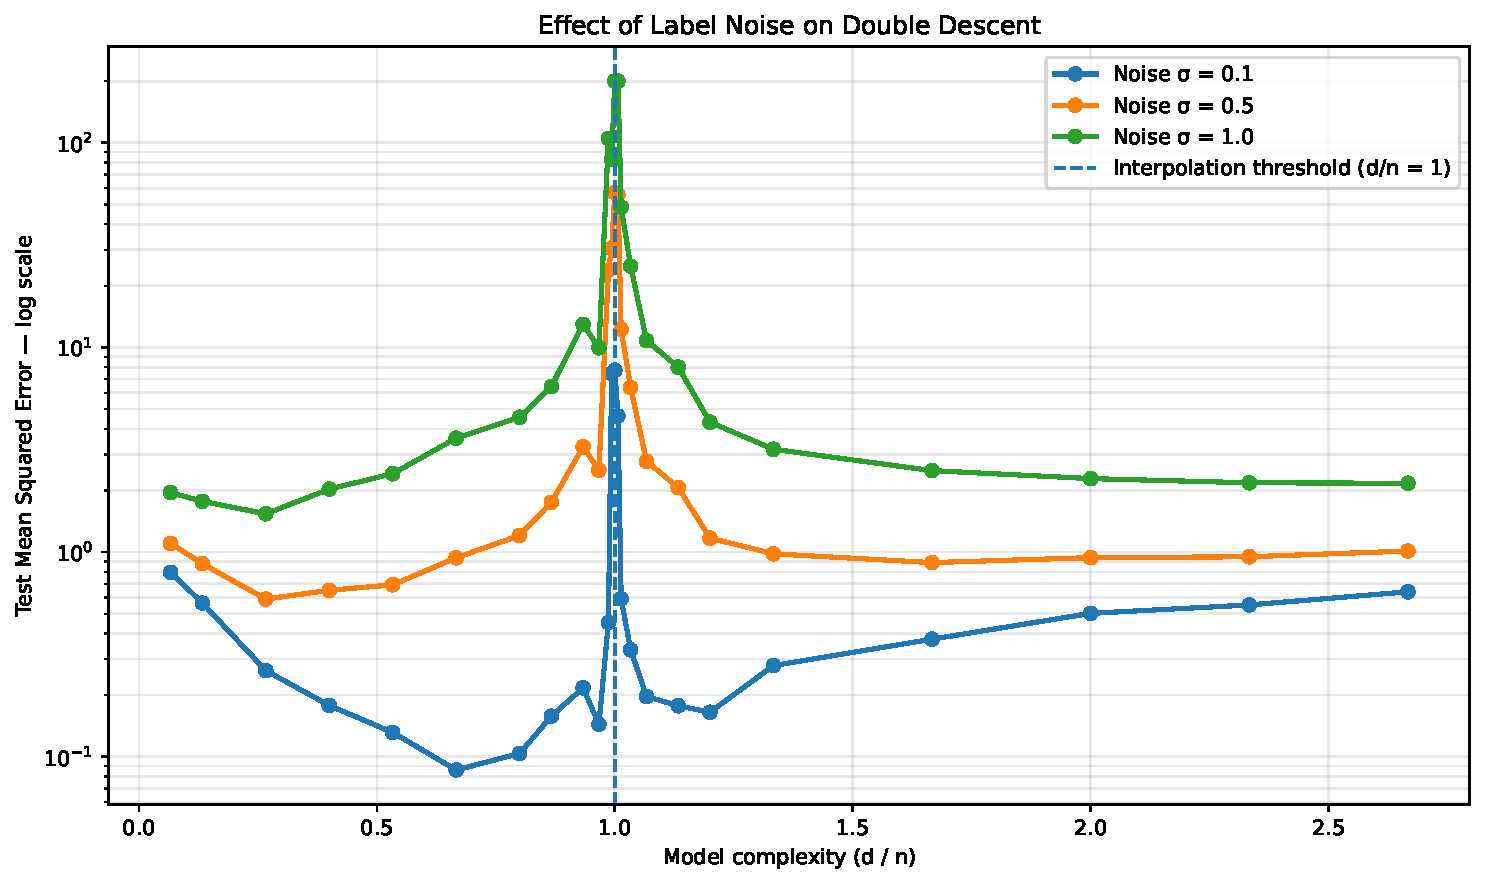
\includegraphics[width=\linewidth,height=0.21\textheight,keepaspectratio]{real_world_07.pdf}
\end{center}
{\small\textit{Figure 6.} The optional synthetic noise extension uses the same seed, feature matrices, coefficient vector and underlying standardized noise draws at each noise level. The displayed errors include test-label noise.}

With seed 42 fixed, the experiment repeats the synthetic sweep at $\sigma\in\{0.1,0.5,1\}$. At $d=150$, test MSE is approximately 7.71, 57.02 and 200.16 respectively. In this diagnostic, larger label noise makes the instability near interpolation more pronounced. The noise variance also changes the irreducible error floor, so the curve's vertical displacement cannot be interpreted as estimation error alone.

This is a single-seed extension. It supports a within-run comparison, but does not establish the same effect size across random datasets. Its seed-42 peak should not be compared numerically with the 30-run mean peak from Figure 1 as if both were the same statistic.

\begin{center}\begin{tabular}{p{0.25\linewidth}p{0.30\linewidth}p{0.30\linewidth}}\toprule
Aspect & Synthetic & Real world\\\midrule
Feature structure & Independent Gaussian & Correlated, sparse, ill-conditioned\\
Signal ordering & Early coordinates designed to matter & Random ordering after filtering\\
Test protocol & Independent same-process samples & One later official test date\\
Threshold & Clear at $d=n$ & Measured residual; varies by run\\
Outcome & Clear double descent & Peak and decline, mixed full-curve evidence\\
\bottomrule\end{tabular}\end{center}

The same solvers can behave very differently under different feature geometry and evaluation protocols. Raw synthetic MSE and log-target BlogFeedback MSE are not on comparable numerical scales. The useful comparison concerns curve shape, interpolation, instability, and response to regularization, rather than which dataset has a smaller MSE.

\newpage
\pageheading{8. Limitations, reproducibility, and conclusions}
\textbf{Numerical sensitivity.} The real-world least-squares fits depend on very small retained singular values. The shared $10^{-10}$ SVD cutoff makes rank reporting consistent with fitting, but it does not eliminate ill-conditioning. Floating-point libraries can produce substantially different least-squares errors near the cutoff. A fresh environment (NumPy 2.5.4, Matplotlib 3.11.2) ran successfully, but one individual near-threshold test error changed by about 40\%; the original results are retained. The ridge/CV extension was stable to negligible numerical differences in that check. Threshold and error magnitudes should therefore be interpreted with the stated tolerances, not as exact symbolic quantities.

\textbf{Exploratory protocol.} The reduction from 150 to 80 training observations was made after inspecting rank and residual behavior. The final results are an exploratory analysis of the revised setup; they are not an untouched-test estimate of a selected prediction procedure. The original curves are descriptive; the extension selects $\alpha$ using training-only cross-validation at each fixed raw dimension. No validation procedure selects $d$. The analysis does not establish that any chosen model would be optimal for future data.

\textbf{Data limitations.} The real-world study uses only a small subset of the available training data and a single held-out date. Correlation, sparse features, and temporal differences may contribute to the observed errors, but the experiment does not isolate their causal contributions. A multi-date evaluation, repeated noise extension, or comparison with a better-conditioned real-world dataset would provide additional evidence. None is claimed here.

\textbf{Reproducible workflow.} The repository provides an executable runner, compatible numerical dependency ranges, both executed notebooks, PNG/PDF exports, numerical JSON files. From the repository root, run:
\begin{verbatim}
python -m pip install -r requirements.txt
python src/run_experiments.py
\end{verbatim}
The verified runtime is Python 3.13.7, NumPy 2.4.6 and Matplotlib 3.11.0. The first run downloads the official dataset only if it is absent; a complete cached dataset permits offline execution. The runner sets the notebook working directory automatically and does not require Jupyter. Detailed environment and runtime information are stored in \texttt{results/environment.json}.

The LaTeX source uses ordinary \texttt{\string\includegraphics} commands to include exported files from \texttt{../figures/}. The source is edited directly; no generator or result-dependent compilation barrier remains. Compile twice with \texttt{pdflatex}, as documented in the README; no BibTeX pass is needed.

\textbf{Conclusions.} Three distinctions are central. First, sufficient parameter count must be separated from observed numerical interpolation. Second, a post-peak decline must be separated from a clean full double-descent curve. Third, improvement over unstable least squares must be separated from performance that beats a meaningful baseline. The synthetic results satisfy the first two strongly. The real-world results verify interpolation but provide mixed evidence for the full curve, and their original final ridge fits fail the baseline comparison. Training-only CV improves ridge but wins against its paired baseline in only 1/20 final comparisons. Reporting these negative findings is essential to an accurate interpretation of the experiment.

\newpage
\pageheading{9. Sources and authorship}
\begin{enumerate}
\item M. Belkin, D. Hsu, S. Ma and S. Mandal (2019). Reconciling modern machine-learning practice and the classical bias--variance trade-off. \textit{Proceedings of the National Academy of Sciences}, 116(32), 15849--15854. \url{https://doi.org/10.1073/pnas.1903070116}.
\item K. Buza (2014). \textit{BlogFeedback} [Dataset]. UCI Machine Learning Repository. \url{https://doi.org/10.24432/C58S3F}. Dataset licensed under Creative Commons Attribution 4.0. The project uses the official archive and the attribution above.
\item N. Cesa-Bianchi. \textit{Machine learning course notes}, supplied course PDF. Relevant material: linear and ridge regression (PDF p. 40) and double descent (PDF p. 68).
\item \textit{Statistical Methods for Machine Learning: Experimental Projects, A.Y. 2025/26}, supplied project brief. Assignment 4 and general coding/report requirements (PDF pp. 1--3, 8--9, 16).
\end{enumerate}

\textbf{Use of AI tools.} AI tools (Codex) were used for code review, implementation revisions, experiment execution, numerical checks, plotting, and report drafting. This assistance applies to the original experiments and the gradient-descent and cross-validation extensions.

% TODO: Check the course's AI policy before submission and confirm that this acknowledgment and declaration comply with it.
% TODO: When rebuilding the PDF, check that the final report is between 5 and 10 pages.
\textbf{Course declaration.}

\begin{quote}\small
I declare that this material, which I now submit for assessment, is entirely
my own work and has not been taken from the work of others, save and to the
extent that such work has been cited and acknowledged within the text of my
work. I understand that plagiarism, collusion, and copying are grave and
serious offences in the university and accept the penalties that would be
imposed should I engage in plagiarism, collusion or copying. This assignment,
or any part of it, has not been previously submitted by me or any other
person for assessment on this or any other course of study.
\end{quote}

\end{document}
